
The previous documents have enlightened how to deal with differential
equation problems, from ordinary to partial derivatives. The idea of this last
document is to go one step further on this scale and give the reader an example
of a mixed problem (it can also be found in the bibliography as 'Initial Value
Boundary Problem'). \\

A mixed problem combines the complexity of Cauchy's and Boundary Value problems,
so one may use the tools and applications described before in order to implement
the software for the new purposes. \\

The description of this problem is presented with an example. Once the example
is understood, one should be able to develop any other problem applying the same
logic and using the software tools available. \\


%1.==========================BODY==============================================
\newpage

\section{Introduction}

The Initial Value Boundary Problem is composed by equations in partial
derivatives which change with time. Usually there is one (or more) parabolic
equation and at least one elliptical equation. Then, the complexity of this
problem mixes the resolution scheme of a Cauchy problem (in order to solve the
temporal evolution) with the procedure for solving a Boundary Problem whose
unknowns change in every time iteration. \\

So, the problem can be written as follows: 

$$\begin{cases}
\frac{d \mathbf{U}}{dt}= \mathbf{F}(\mathbf{U},\mathbf{V}, t) \hspace{1cm} +ICs,
+BCs\\

\mathbf{H}(\mathbf{U},\mathbf{V})=0 \hspace{1.6cm} +BCs\\
\end{cases}
$$

where $\mathbf{U}$ are the unknown variables of the problem with explicit
temporal derivatives and $\mathbf{V}$ are the others (which certainly change
with time but the derivative is not explicit in the equations).
\\

The resolution problem can be summarized as follows: 

Beginning with the initial condition ($\mathbf{U} (t=0)= \mathbf{U_0}$),
$\mathbf{V}$ is calculated from the elliptical equation
$\mathbf{H}(\mathbf{U},\mathbf{V}, t)=0 $. Once $\mathbf{V}$ is known, with the
initial values of $\mathbf{U}$ and $\mathbf{V}$ we are able to evaluate
$\mathbf{F}(\mathbf{U},\mathbf{V})$ and advance one time step using any temporal
scheme. Then the process is restarted with the new $\mathbf{U}$ that has been
calculated. \\

\begin{framed}

\framebox[3cm]{$\begin{array}{c} 
\text{Inital condition},\\
\mathbf{U} (t=0)= \mathbf{U_0} \end{array}$}

\hspace{1.5 cm}$\Downarrow$

\framebox[3cm]{$ \hspace{0.2cm} \begin{cases}
\mathbf{H}(\mathbf{U^n},\mathbf{V})=0
\\
+BCs
\end{cases}$}  
 $\Rightarrow \mathbf{V^n} \Rightarrow $
\framebox[4cm]{$ \hspace{0.2cm} \begin{cases}
\frac{d \mathbf{U}}{dt}= \mathbf{F}(\mathbf{U^n},\mathbf{V^n}, t^n)
\\
+BCs
\end{cases}$}  
 $\Rightarrow \frac{d \mathbf{U^n}}{dt} \Rightarrow $
 \framebox[4cm]{ $\begin{array}{c} 
 
 \text{Temporal scheme}, \\
 
 \mathbf{U^{n+1}}=\mathbf{F}(\mathbf{U^n},\frac{d \mathbf{U^n}}{dt})
 \end{array}$}\\
 
  \hspace{1.5 cm}$\Uparrow$ \hspace{10.5cm} $\Downarrow$
 
\framebox[3cm]{$\mathbf{U^n}$}  \hspace{0.5cm} $\Leftarrow$
\hspace{0.5cm} 
\framebox[4cm]{$t^n = t_0 +n\cdot \Delta t$} 
\hspace{0.5cm} $\Leftarrow$ \hspace{0.5cm}
\framebox[4cm]{$n=n+1$}

\end{framed}

\vspace{1cm}

In order to understand the procedure to solve this kind of problems an example
is presented: the flow inside a square cell, with different temperatures in the
walls. One will see the numerical method (as presented in the chart above) and
some details and particularities which may be interesting in order to show the
capabilities of the software.\\

 In the following section, the problem is presented and then the numerical
 approach to it is explained. \\


\newpage

\section{Convection cell}

The problem presented as example is known in the bibliography as 'Convection
cell'. There is a fluid inside an square box, let's assume the fluid is
incompressible; and the walls may have different boundary conditions. Let one
wall be 'hot' ($T_{hot}$), the opposite one 'cold' ($T_{cold}$) and the two
remaining, adiabatic ($\frac{\delta T}{\delta n}=0$).\\

\begin{figure}[h]
\centering
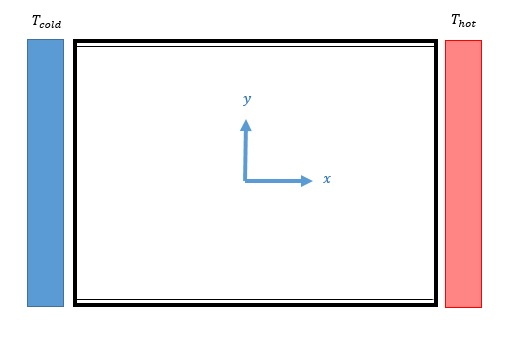
\includegraphics[scale=0.8, trim = 5mm 0mm 0mm 0mm, clip]{./Figures/4-IVBP/figure_0.jpg}
\caption{The convection cell}
\end{figure}

The equations for this problem are: 

\begin {equation} \label{cont}
\nabla \cdot \mathbf{v}= 0
\end{equation}

\begin {equation} \label{cdm}
\rho \cdot \left( \frac{\delta \mathbf {v}}{\delta t} + \mathbf{v} \cdot
\nabla \mathbf{v}\right)= -\nabla P + \mu \cdot \nabla^2 \mathbf{v} + \rho g
\beta T (-\mathbf{j})
\end{equation}

\begin {equation} \label{ener}
\rho c_p \cdot \left( \frac{\delta T}{\delta t} + \mathbf{v} \cdot
\nabla T\right)= k \cdot \nabla^2 T + q
\end{equation}

The first difficulty to solve this problem is the boundary condition in the
pressure field ($P$), which is not evident. An alternative path to this problem
is working in terms of the stream function \ref{stream_function} and
vorticity \ref{vorticity}. \\

\begin {equation} \label{stream_function}
u=\frac{\delta \Psi}{\delta y}, \hspace{0.5cm} v=-\frac{\delta \Psi}{\delta x},
\end{equation}

\begin{equation} \label{vorticity}
\omega= \nabla \times \mathbf{v}
\end{equation}

Then, the equations \ref{vorticity} and \ref{cdm} can be written as follows
\footnote{The continuity equation is no longer needed because the stream function ensures its compliance.}:

\begin {equation} \label{cont2}
\omega= - \nabla^2 \Psi
\end{equation}

\begin {equation} \label{cdm2}
\rho \cdot \left( \frac{\delta \omega}{\delta t} + \mathbf{v} \cdot
\nabla \omega\right)=  \mu \cdot \nabla^2 \omega - \rho g
\beta \frac{\delta T}{\delta x}
\end{equation}

With this new approach, the unknown functions of the problem are scalar
fields (in fact the vorticity is vectorial but in a 2D problem only the normal
component plays a roll in the flow), the boundary conditions can be imposed on
the stream function and temperature and the pressure is hidden in this
formulation. \\

A second difficulty appears however, once again concerning the boundary
conditions. As we are to solve the problem inside a closed box, the velocity of
the fluid is assumed zero for the fluid in contact with the walls. These
boundary conditions lead to eight equations in the stream function ($u=v=0$ in
$\delta \Omega$, that is to say in each of the four walls), while there is no
boundary condition in the vorticity. This difficulty will be dealed later when
explaining the numerical approach to the problem. \\

\vspace{1 cm}

So, for this problem three equations are needed \ref{cont2}, \ref{cdm2},
\ref{ener}, for the three scalar fields $\Psi$, $\Omega$ and $T$. Plus, one
can also compute the velocity from the definition of the stream function
\ref{stream_function}, but this is not essential. \\

Now, as usual when working with fluids, let's transform the equations to
non-dimensional variables. \\



\subsection{Non-dimensional equations}

First of all some magnitudes are to be defined: 

\begin{itemize}
  \item Characteristic dimension: the length of the walls $2a$: $x=(2a)\hat x$, 
  $y=(2a)\hat y$.
  \item Characteristic velocity $u_c$ \footnote{Sometimes, in this kind of problems the
  characteristic velocity is written as $u_c= \frac{k}{\rho c_p (2a)}$, which
  is useful for simplifying  the problem.}: $u= u_c \cdot \hat u$, $v=
  u_c \cdot \hat v$ .
  \item Temperature $\theta= \frac{T-T_{cold}}{T_{hot}-T_{cold}}$.
  \item Time $t= \frac{(2a)}{u_c} \hat t$
\end{itemize}

and three characteristic numbers appears: 

\begin{itemize}
  \item Reynolds $Re \sim \frac{\rho u_c (2a)}{\mu}$ \footnote{If $u_c=
  \frac{k}{\rho c_p (2a)}$, then $Re \sim 1/Pr$}.
  
  \item Prandtl $Pr \sim \frac{\mu c_p}{k}$.
  \item Rayleigh $Ra \sim \frac{g \beta (T_{hot}-T_{cold})}{\frac{\mu}{\rho}
  \frac{k}{\rho c_p}}\cdot (2a)^3$
\end{itemize}

So the equations are: 

\begin {equation} \label{cont3}
\omega= - \left( \frac{\delta^2 \Psi}{\delta x^2} + \frac{\delta^2
 \Psi}{\delta y^2} \right)
\end{equation}

\begin {equation} \label{cdm3}
 \frac{\delta \omega}{\delta t} = -u \cdot \frac{\delta \omega}{\delta x} -v
 \cdot \frac{\delta \omega}{\delta y} +
 \frac{1}{Re} \cdot \left( \frac{\delta^2 \omega}{\delta x^2} + \frac{\delta^2
 \omega}{\delta y^2} \right) - \frac{Ra}{Pr \cdot Re^2}
\frac{\delta \theta}{\delta x}
\end{equation}

\begin {equation} \label{ener3}
 \frac{\delta \theta}{\delta t} =  -u \cdot \frac{\delta \theta}{\delta x} -v
 \cdot \frac{\delta \theta}{\delta y}+ \frac{1}{Re \cdot Pr} \cdot \left(
 \frac{\delta^2 \theta}{\delta x^2} + \frac{\delta^2 \theta}{\delta y^2} \right)
\end{equation}


Where all the variables are non-dimensional ( $\hat{\phi}$ has been omitted for
simplifying the writing).

\subsection{Boundary conditions}

We have pointed that there is a difficulty concerning the boundary conditions.
As we have said, eight boundary conditions applies to the stream function while
no condition is applied to the vorticity. \\

The conditions for the stream function comes from assuming zero velocity of the
fluid in contact with the walls. Then, 

\begin{equation}
u(x,y)=v(x,y)=0, \hspace{1cm} (x,y)\in \delta \Omega
\end{equation}

\begin{equation}
\frac{\delta \Psi}{\delta y} (x,y)= \frac{\delta \Psi}{\delta x} (x,y)=0,
\hspace{1cm} (x,y)\in \delta \Omega
\end{equation}

It can also be written as follows: 

\begin{equation}
\frac{\delta \Psi}{\delta \mathbf{s}} (x,y)= \frac{\delta \Psi}{\delta
\mathbf{n}} (x,y)=0, \hspace{1cm} (x,y)\in \delta \Omega
\end{equation}

Where $\mathbf{s}$ and $\mathbf{n}$ are the coordinates along the wall and
normal to it, respectively.\\

The boundary conditions for the temperature can be arbitrary. One can choose
two walls with different temperatures and the remaining ones, adiabatic:

\begin{equation}
T=T_{cold} \rightarrow \theta=0, \hspace{1cm}
(x,y)\in(-a,y)
\end{equation}

\begin{equation}
T=T_{hot} \rightarrow \theta=1, \hspace{1cm}
(x,y)\in(+a,y)
\end{equation}

\begin{equation}
\frac{\delta T}{\delta \mathbf{n}}=0 \rightarrow \frac{\delta \theta}{\delta
\mathbf{n}}=0, \hspace{1cm} (x,y)\in(x,\pm b)
\end{equation}\\ 

\begin{figure}[h]
\centering
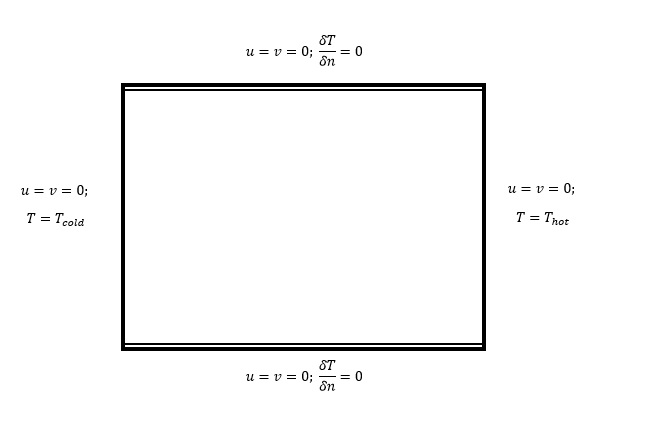
\includegraphics[scale=0.8, trim = 5mm 10mm 0mm 10mm,
clip]{./Figures/4-IVBP/figure_1.jpg}
\caption{Spatial domain and boundary conditions}
\label{BC_figure}
\end{figure}

The boundary conditions for the vorticity will be taken from the equation
\ref{cont3} once the stream function is known. The solving process can be
summarized as follows: 

\begin{itemize}
  \item Assuming the vorticity is known in the interior points of the domain (at
  the beginning from the initial condition and then from the previous time step), the stream function is
  calculated with \ref{cont3}: 
$$ \omega= - \left( \frac{\delta^2 \Psi}{\delta x^2} + \frac{\delta^2
 \Psi}{\delta y^2} \right) \rightarrow \Psi=\Psi(x,y)$$
 \item Then, the vorticity in the boundaries of the spatial domain is calculated
 with this same equation: 
 $$ \omega_{\delta \Omega}= - \left( \frac{\delta^2 \Psi}{\delta
 x^2} + \frac{\delta^2 \Psi}{\delta y^2} \right)_{\delta \Omega} \rightarrow
 \omega_{\delta \Omega}=\omega(x,y) \hspace{0.5cm} (x,y) \in \delta \Omega$$
 \item These values are used as boundary conditions for the evolution problem
 (equation \ref{cdm3}).
\end{itemize} 


Now, let's look into the numerical approach to this problem. \\

\newpage

\section{Numerical approach to the problem}

First of all the equations will be discretized. The notation we have used is: 

$$\theta(x,y,t) \rightarrow \theta^{ij} = \theta(i,j)_n$$

Where $i,j$ are the index of the spatial mesh ($x_i, y_j$) and $n$ refers to the
time step ($t=t_0+n\cdot \Delta t$). \\

The discretized equations are: 

\begin {equation} \label{cont4}
\omega^{ij}= - (\Psi^{ij} _{xx} + \Psi^{ij} _{yy})
\end{equation}

\begin {equation} \label{cdm4}
 \frac{\delta \omega^{ij}}{\delta t} = -\Psi^{ij} _{y} \cdot 
 \omega^{ij}_x + \Psi^{ij} _{x} \cdot \omega^{ij}_y +
 \frac{1}{Re} \cdot ( \omega^{ij}_{xx} + \omega^{ij}_{yy}) - \frac{Ra}{Pr \cdot
 Re^2} \cdot \theta^{ij}_x
\end{equation}

\begin {equation} \label{ener4}
 \frac{\delta \theta^{ij}}{\delta t} =  -\Psi^{ij} _{y} \cdot 
 \theta^{ij}_x + \Psi^{ij} _{x} \cdot \theta^{ij}_y + \frac{1}{Re \cdot Pr}
 \cdot ( \theta^{ij}_{xx} + \theta^{ij}_{yy})
\end{equation}

The boundary conditions: 

\begin{equation} \label{BCs1}
 \Psi^{ij}_ \mathbf{s}= \Psi^{ij}_ \mathbf{n}=0, \hspace{1cm} (i,j)\in \delta
 \Omega
\end{equation}

\begin{equation} \label{BCs2}
 \omega^{ij} = f(\Psi^{ij}), \hspace{1cm} (i,j)\in \delta
 \Omega
\end{equation}

\begin{equation} \label{BCs3}
 \theta^{ij}_ \mathbf{n}=0, \hspace{1cm} (i,j)\in
 \delta \Omega_0
\end{equation}

\begin{equation} \label{BCs4}
 \theta^{ij} =0, \hspace{1cm} (i,j)\in
 \delta \Omega_1
\end{equation}

\begin{equation} \label{BCs5}
 \theta^{ij} =1, \hspace{1cm} (i,j)\in
 \delta \Omega_2
\end{equation}

And the initial conditions: 

\begin{equation} \label{IC1}
 \omega^{ij} = \omega^{ij}_0, \hspace{1cm} (i,j)\in  \Omega
\end{equation}

\begin{equation} \label{IC2}
 \theta^{ij} = \theta^{ij}_0, \hspace{1cm} (i,j)\in  \Omega
\end{equation}

\subsection{Solving procedure}

\begin{framed}

\framebox[3cm]{$\begin{array}{c} 
\text{Inital condition},\\
\omega^{ij}_0  \hspace{0.5cm}\text{eq. [\ref{IC1}]}\end{array}$}

\hspace{1.5 cm}$\Downarrow$

\framebox[3cm]{$ \hspace{0.2cm} \begin{cases}
\text{BVP eq.[\ref{cont4}]}\\
\text{+ BCs eq.[\ref{BCs1}]}
\end{cases}$}  
 $\Rightarrow \Psi^{ij} \Rightarrow $
\framebox[4cm]{$ \hspace{0.2cm} \begin{cases}
\text{Cauchy  eq.[\ref{cdm4} \ref{ener4}] }\\
\text{+ BCs eq.[\ref{BCs2} \ref{BCs3} \ldots]}
\end{cases}$}  
 $\Rightarrow \frac{d \mathbf{U^n}}{dt} \Rightarrow $
 \framebox[4cm]{ $\begin{array}{c} 
 
 \text{Temporal scheme}, \\
 
 \mathbf{U^{n+1}}=\mathbf{F}(\mathbf{U^n},\frac{d \mathbf{U^n}}{dt})
 \end{array}$}\\
 
  \hspace{1.5 cm}$\Uparrow$ \hspace{10.5cm} $\Downarrow$
 
\framebox[3cm]{$\mathbf{\omega_{n}^{ij}}$}  \hspace{0.5cm}$\Leftarrow$
\hspace{0.5cm} \framebox[4cm]{$t^n = t_0 +n\cdot \Delta t$} 
\hspace{0.5cm} $\Leftarrow$ \hspace{0.5cm}
\framebox[4cm]{$n=n+1$}


\end{framed}


\newpage
\subsection{Boundary value problem}

As we have seen, with the vorticity field from the previous iteration we can
solve the boundary value problem and find the new stream function. The equations
are: 

\begin {equation} \label{cont4}
\omega^{ij}= - (\Psi^{ij} _{xx} + \Psi^{ij} _{yy})
\end{equation}

\begin{equation} \label{BCs10}
 \Psi^{ij}_ \mathbf{s}= \Psi^{ij}_ \mathbf{n}=0, \hspace{1cm} (i,j)\in \delta
 \Omega
\end{equation}

The important thing to remark here is that eight conditions are to be applied
while only four are necessary to solve the Poisson problem. As we have explained
this is because there are four of this conditions that substitute the unknown
boundary conditions of the vorticity. \\

In order to solve this problem, first of all let's look into the discretized
boundary conditions using finite differences as usual. Then, the derivative is
transformed to a polynomial expression depending on the function value of the
nearby points. For example in the wall at $x=-a$ ($i=0$):

\begin{equation} \label{BCs101}
 \Psi^{0,j}_ \mathbf{s} = f(\Psi^{0,j-n} \ldots \Psi^{0,j} \ldots \Psi^{0,j+n}
 )=0
\end{equation}

\begin{equation} \label{BCs102}
 \Psi^{0,j}_ \mathbf{n} = f(\Psi^{0,j}, \Psi^{1,j} \ldots \Psi^{n,j} )=0
\end{equation}\\

\begin{figure}[h]
\centering
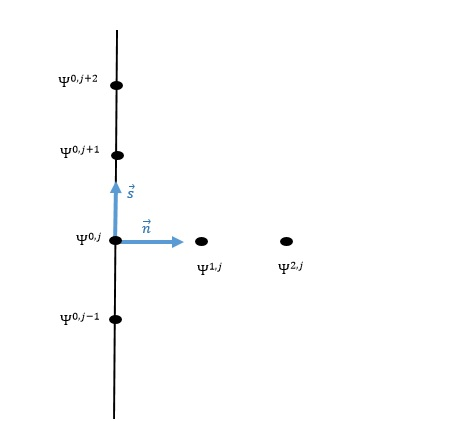
\includegraphics[scale=1, trim = 5mm 0mm 30mm 10mm,
clip]{./Figures/4-IVBP/figure_2.jpg}
\caption{Boundary conditions for the stream function}
\label{BC_figure_2}
\end{figure}


The equations \ref{BCs101} and \ref{BCs102} can be rewritten as follows: 

\begin{equation} \label{BCs103}
 \Psi^{0,j} = f(\Psi^{0,j-n} \ldots \Psi^{0,j+n})
\end{equation}

\begin{equation} \label{BCs104}
 \Psi^{1,j}= f(\Psi^{0,j}  \ldots \Psi^{n,j} )
\end{equation}\\

Proceeding the same way in the other walls we will get enough equations for the
function values in the boundary points and the following ones. Then, the Poisson
problem is to be solved in the interior points (inside the dashed square in the
figure):

\begin {equation} \label{cont5}
\omega^{ij}= - (\Psi^{ij} _{xx} + \Psi^{ij} _{yy}) \hspace{1cm} (i,j) \in
(2:Nx-2, 2:Ny-2)
\end{equation}

\begin{figure}[h]
\centering
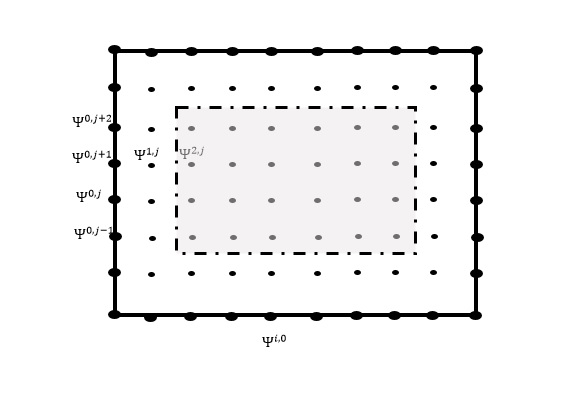
\includegraphics[scale=1, trim = 5mm 10mm 10mm 0mm, clip]{./Figures/4-IVBP/figure_3.jpg}
\caption{Boundary value problem}
\label{BVP}
\end{figure}

For this purpose a special extension of the boundary value problem application
has been prepared. This subroutine allows the user to work with the two boundary
conditions in each wall while the differential equation is applied only in a
square of dimension $(2:N-2)\times(2:N-2)$: 

\begin{blueframed}
\begin{lstlisting}
subroutine multiBC_Boundary_Value_Problem2D(x_nodes, y_nodes, &
		Order, Differential_operator, &
		Boundary_conditions1, Boundary_conditions2, &
		Solution)

     real, intent(inout) :: x_nodes(0:), y_nodes(0:)
     integer, intent(in) :: Order
     procedure (DifferentialOperator2D) :: Differential_operator
     procedure (BC2D) ::  Boundary_conditions1
     procedure (BC2D) ::  Boundary_conditions2
     real, intent(out) :: Solution(:,:)

\end{lstlisting}
\end{blueframed}

However, from the application layer the user should call the routine as usual
just applying two sets of boundary conditions (the easiest way is to define the
conditions on $s$ in one function and the ones in $n$ in a different one).\\

\begin{blueframed}
\begin{lstlisting}
call Boundary_Value_Problem(x_nodes= x_nodes, y_nodes= y_nodes,&
		 Order = Order, &
                 Differential_operator = Equation,  &
                 Boundary_conditions1 = BCs1, &
                 Boundary_conditions2 = BCs2, Solution = FF )
\end{lstlisting}
\end{blueframed}


\begin{blueframed}
\begin{lstlisting}
real function BCs1(x, y, u, ux, uy)
           real, intent(in) :: x, y, u, ux, uy


   if (x==x_nodes(0)) then
                      BCs1 = uy
   elseif (y==y_nodes(0)) then
                      BCs1 = ux
   elseif (x==x_nodes(Nx)) then
                      BCs1 = uy
   elseif (y==y_nodes(Ny)) then
                      BCs1 = ux
   else
        write(*,*) " Error BCs x=", x
        write(*,*) " a, b=", a, b
        read(*,*)
   endif

end function

real function BCs2(x, y, u, ux, uy)
           real, intent(in) :: x, y, u, ux, uy


   if (x==x_nodes(0)) then
                      BCs2 = ux
   elseif (y==y_nodes(0)) then
                      BCs2 = uy
   elseif (x==x_nodes(Nx)) then
                      BCs2 = ux
   elseif (y==y_nodes(Ny)) then
                      BCs2 = uy
   else
        write(*,*) " Error BCs x=", x
        write(*,*) " a, b=", a, b
        read(*,*)
   endif

end function
\end{lstlisting}
\end{blueframed}

\subsection{Cauchy Problem}

The boundary condition for the vorticity is calculated from the stream function: 

\begin {equation} \label{BCs200}
\omega^{ij}= - (\Psi^{ij} _{xx} + \Psi^{ij} _{yy}) \hspace{1cm} (i,j)\in \delta \Omega
\end{equation}

And the evolution problem for the interior points is to be written as usual,
with the equations \ref{cdm4}, \ref{ener4}:

\begin {equation} \label{Cauchy}
\frac{d \mathbf{X}}{dt}= \mathbf{F} (\mathbf{X}) 
\end{equation}

\begin {equation} \label{Cauchy2}
\frac{d}{dt} \left \{ {\begin{array}{c} \omega^{ij} \\ \theta^{ij} \end{array}}
\right \}= \left \{ {\begin{array}{c} F_{xy} (\omega^{ij}, \Psi^{ij},
\theta^{ij}) \\
T_{xy}(\Psi^{ij}, \theta^{ij})
\end{array}} \right \}
\end{equation}


So a transformation is needed from the matrix $\omega^{ij}$, $\theta^{ij}$ to the vector $X$: 

\begin{blueframed}
\begin{lstlisting}
	X(1:M)=reshape(WW, [ M ]);
	X(M+1:2*M)=reshape(TT, [ M ]);
\end{lstlisting}
\end{blueframed}

Where $M$ is the total amounts of nodes: $M=(N_x+1)\cdot(N_y+1)$. \\

However it is more comfortable to us to work with $WW(i,j)$ and $TT(i,j)$ rather
than $X(k)$. So each time step we will transform the vector, calculate the
operator $F$ and then return this operator with the appropriate structure: 

\begin{blueframed}
\begin{lstlisting}
	WW = reshape( X(1:M), [Nx+1, Ny+1] )
	TT = reshape ( X(M+1:2*M), [Nx+1, Ny+1] )
	
	!call BVP for the stream function
	!...(calculation of the operator F)
	
	F(1:M)=reshape(Fxy, [ M ] );
	F(1+M:2*M)=reshape(Txy, [ M ] );
\end{lstlisting}
\end{blueframed}


\begin{blueframed}
\begin{lstlisting}
 call Cauchy_Problem_Solution( Domain = T_Domain, &
 		Initial_C = vorticity_IC, &
		System = System_1, &
		Scheme= Runge_Kutta4, &
		Outputs = vorticity_graphs)
\end{lstlisting}
\end{blueframed}

\newpage

\section{Results}

With the aim of testing the application, a model is prepared with the following
parameters:

$$\text{Characteristic velocity:   }\hspace{0.5cm} u\sim \frac{k}{\rho c_p
(2a)}$$ $$\text{Reynolds number:   }\hspace{0.5cm} Re= \frac{\rho u (2a)}{\mu} \sim
\frac{1}{Pr}
$$
$$\text{Prandtl number:   }\hspace{0.5cm} Pr= \frac{\mu c_p }{k} \sim 1
$$
$$\text{Rayleigh number:   }\hspace{0.5cm} Ra= \frac{g \beta
(T_{hot}-T_cold)}{\frac{\mu}{\rho} \frac{k}{\rho c_p}} (2a)^3 \sim 10^5 $$


The following figures present the results obtained of the test case.

\begin{multicols}{2}

\begin{figure}[H]
\centering
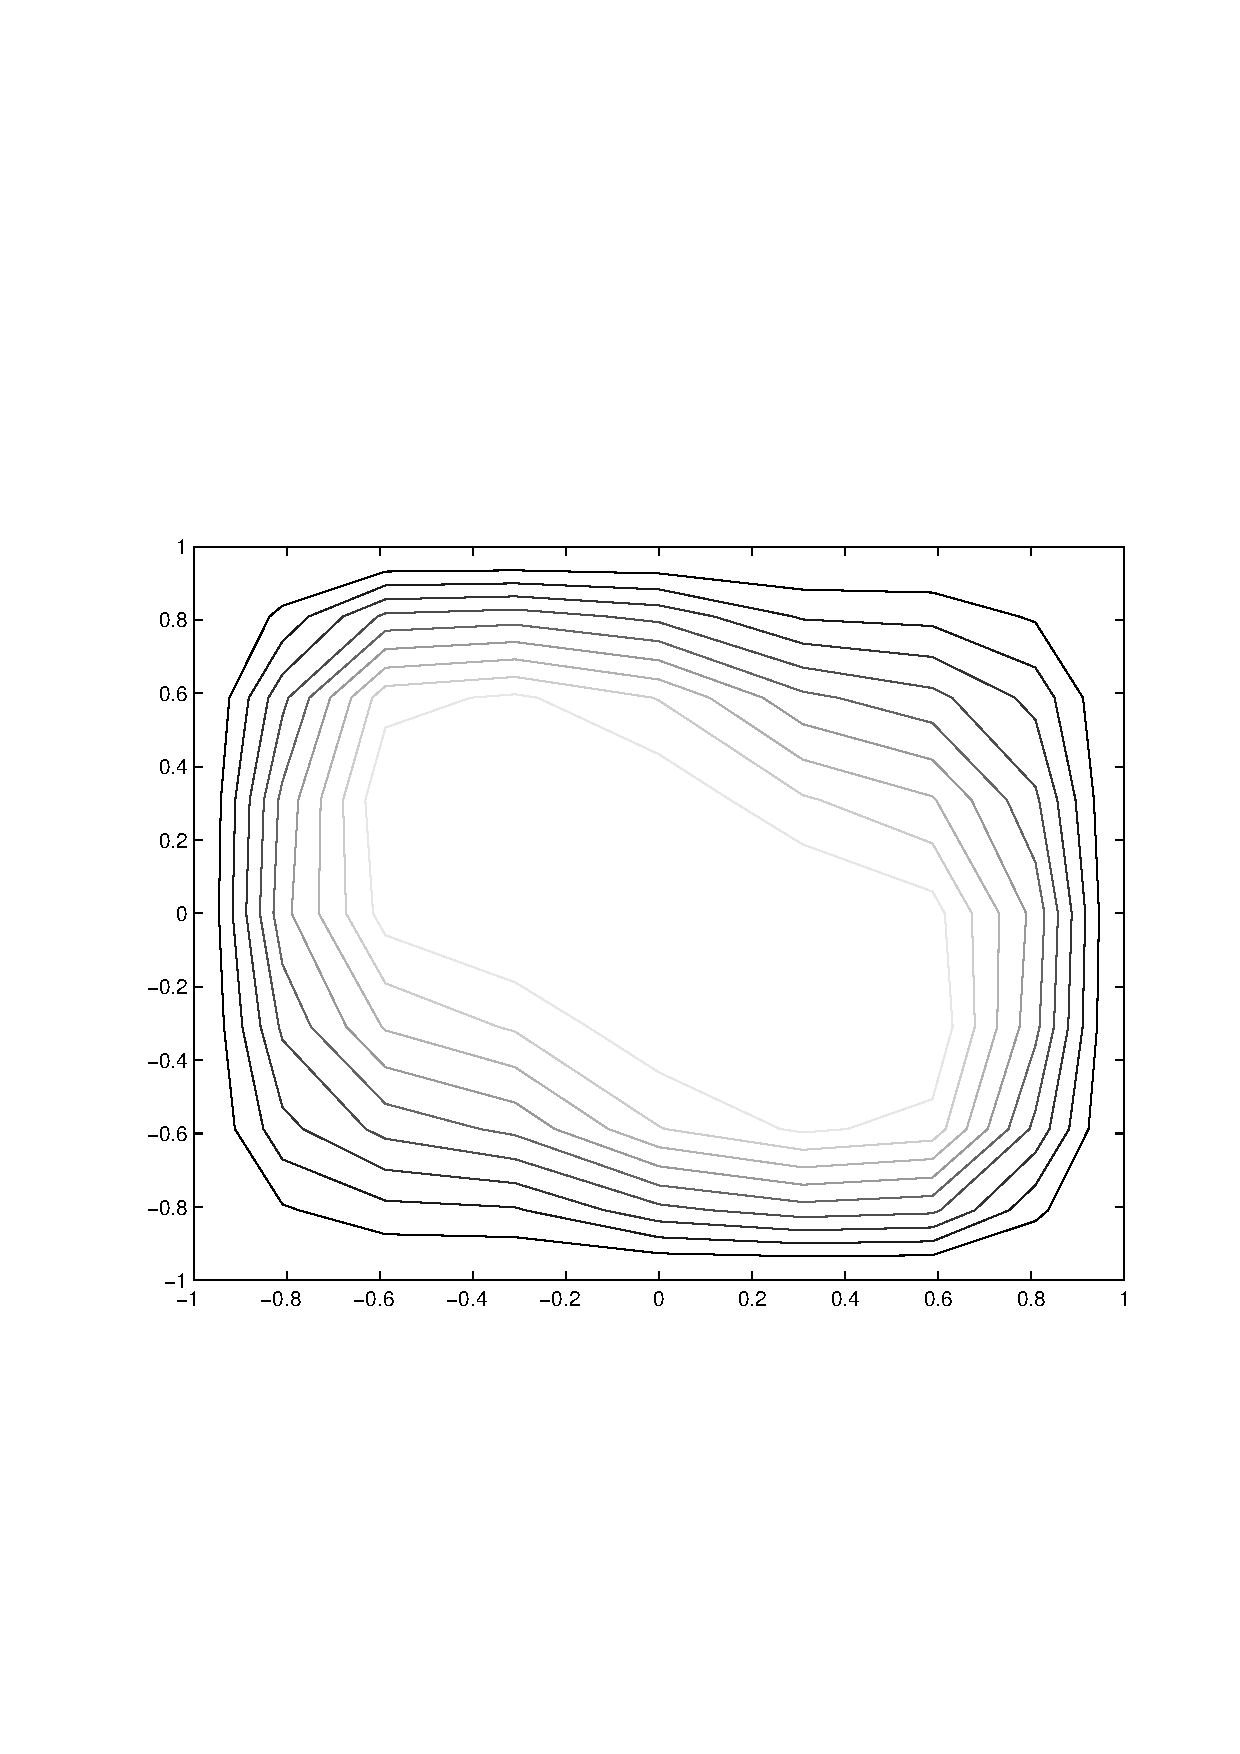
\includegraphics[scale=0.45, trim = 30mm 75mm 15mm 80mm, clip]{./Figures/4-IVBP/stream_t_1.pdf}
\caption{Stream function isolines, $t=0.1$.
}
\end{figure}


\columnbreak

\begin{figure}[H]
\centering
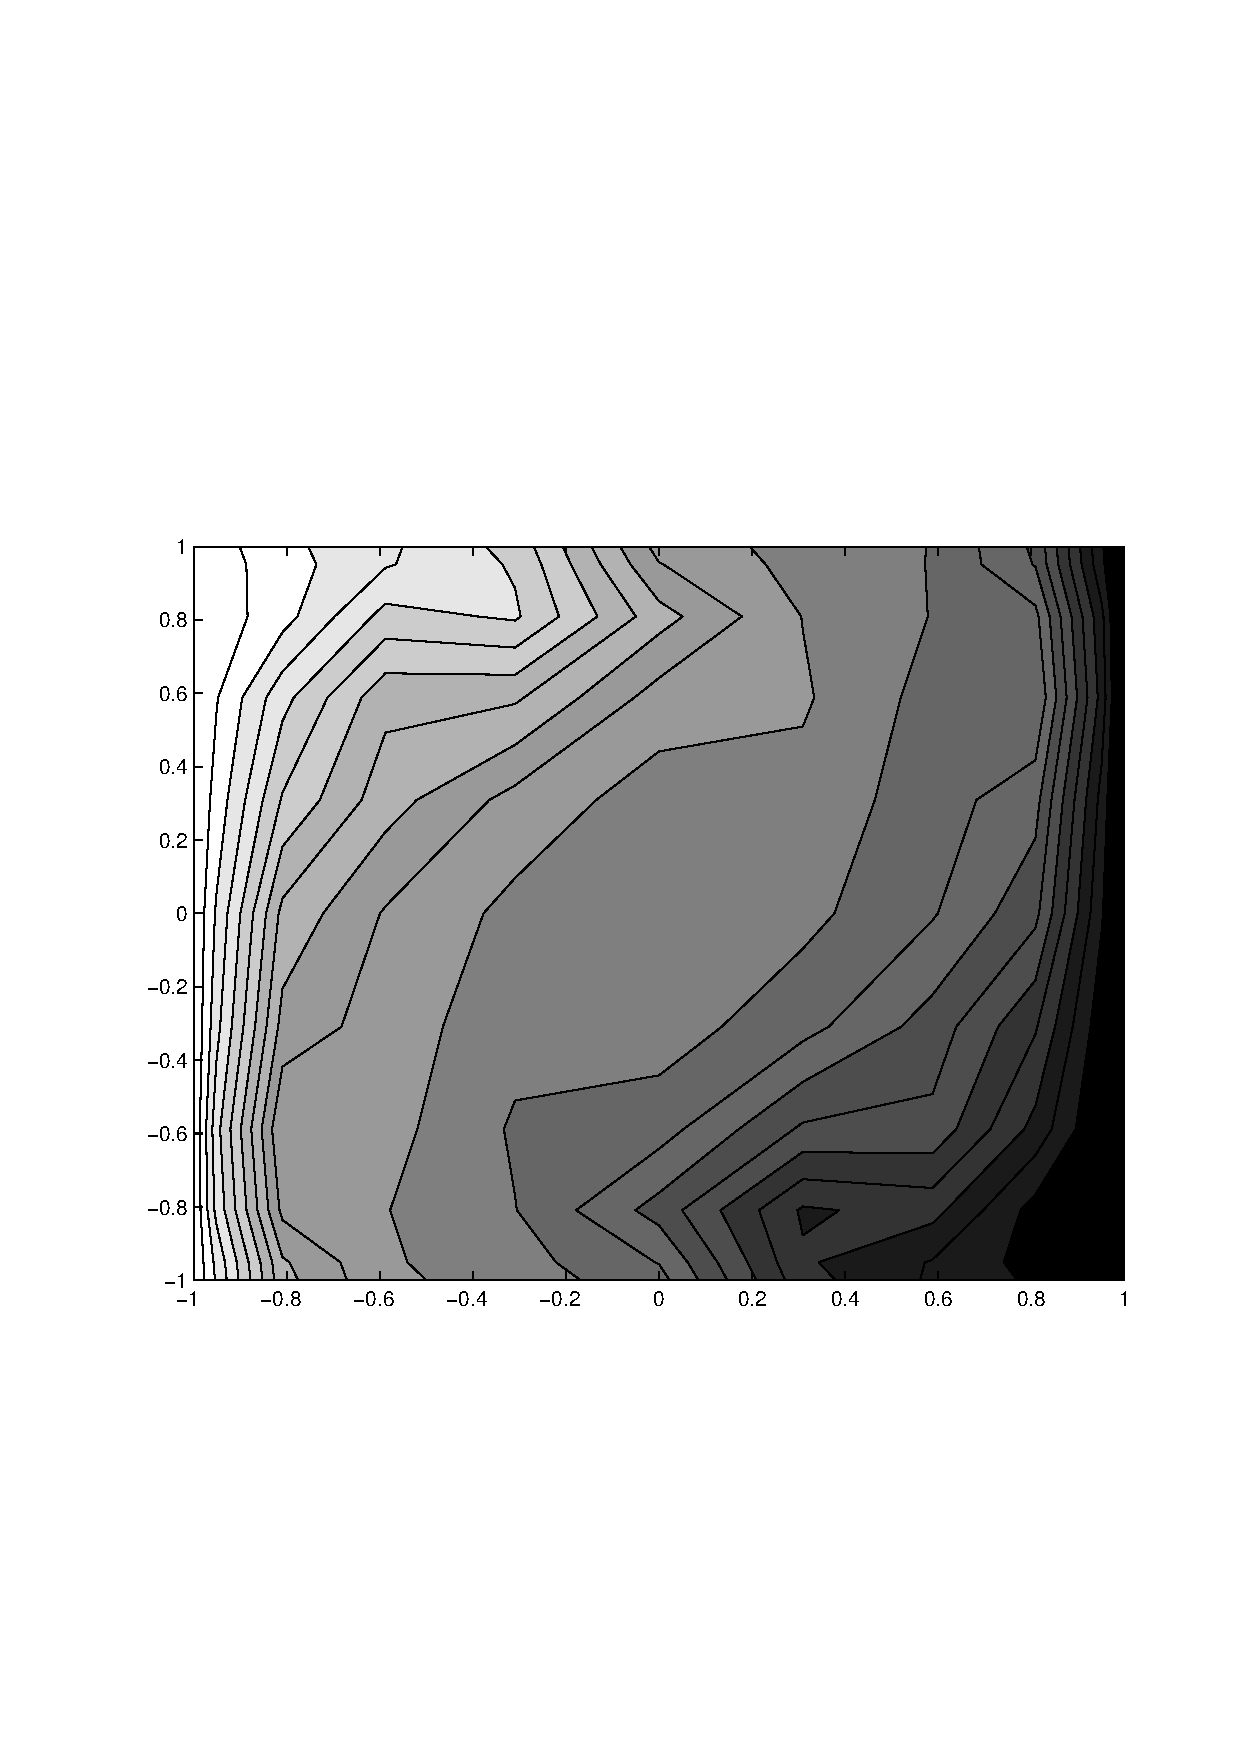
\includegraphics[scale=0.45, trim = 30mm 75mm 15mm 80mm,
clip]{./Figures/4-IVBP/temperature_t_1.pdf} \caption{Temperature contours, $t=0.1$.}
\end{figure}

\end{multicols}

\begin{multicols}{2}

\begin{figure}[H]
\centering
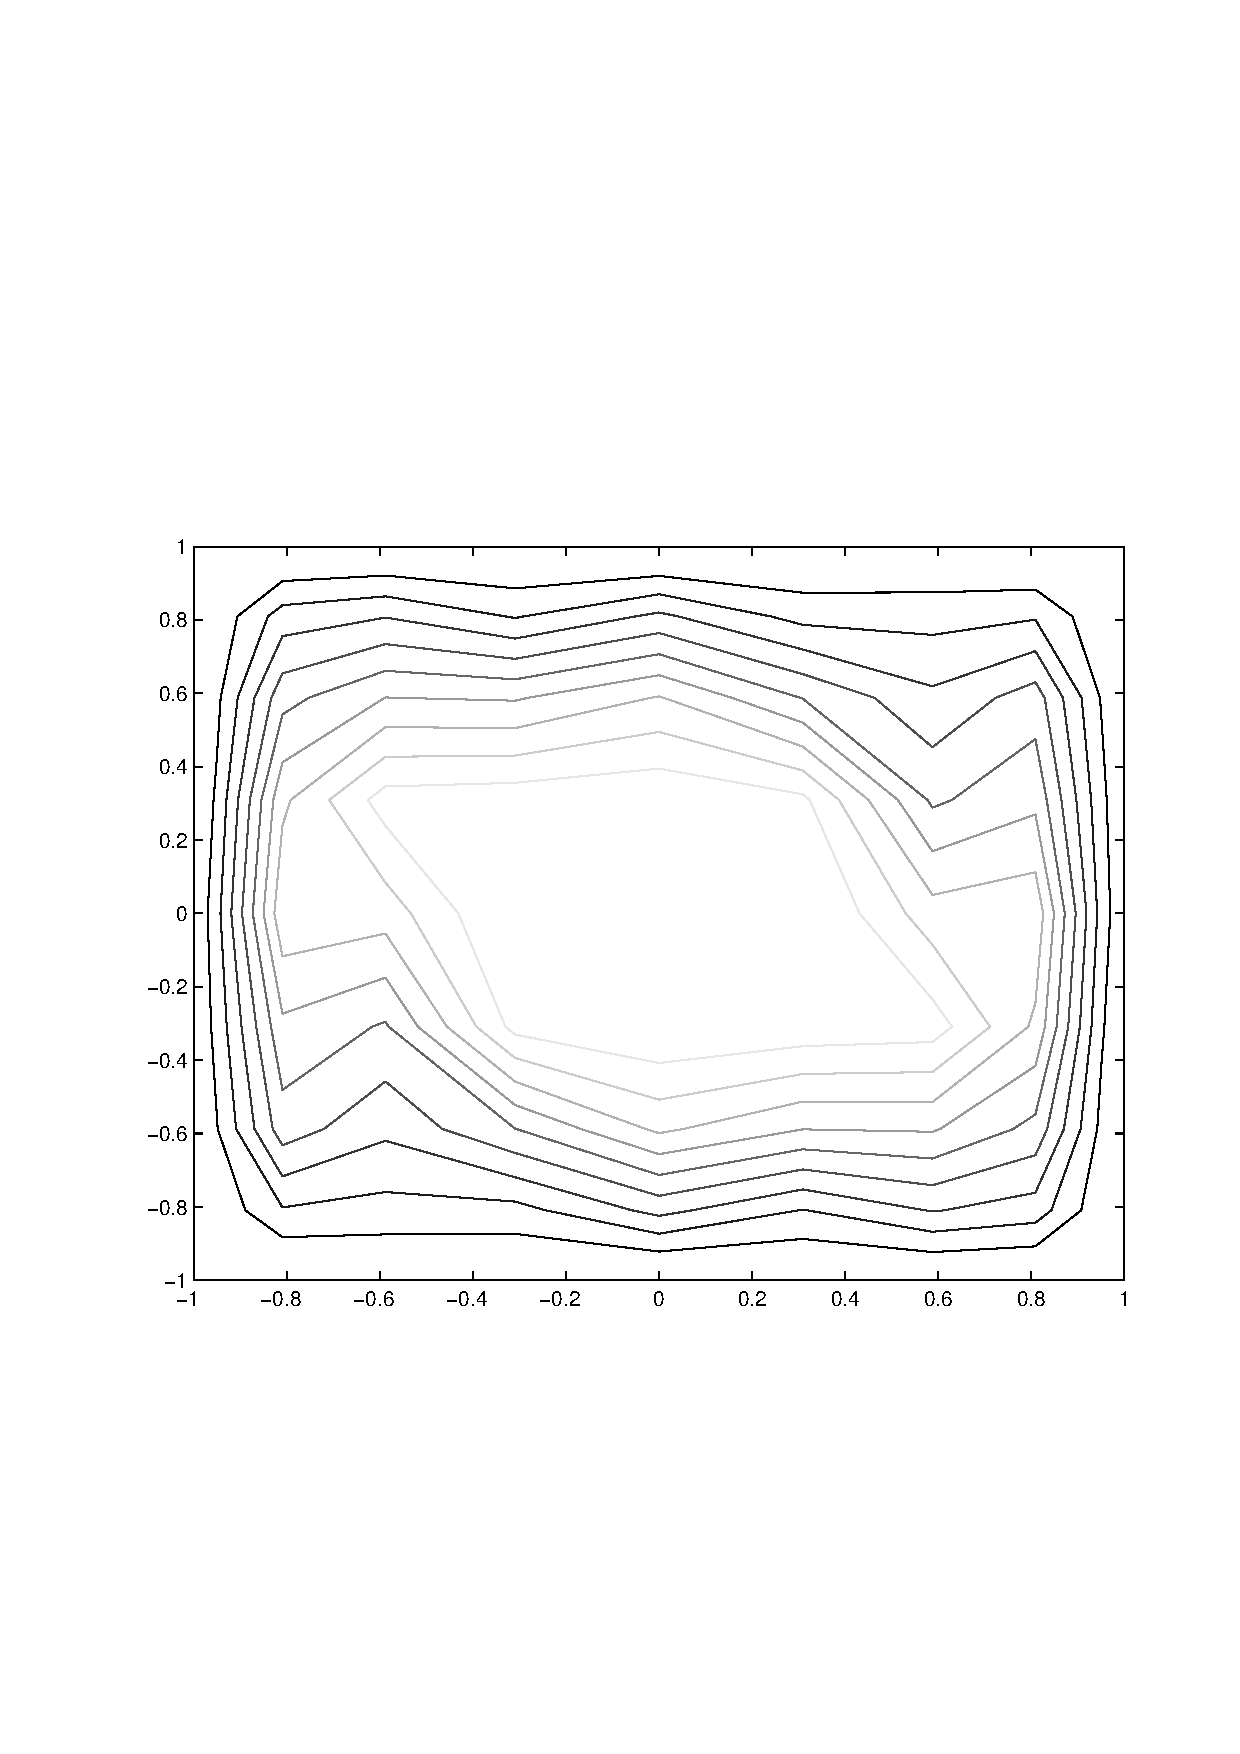
\includegraphics[scale=0.45, trim = 30mm 75mm 15mm 80mm, clip]{./Figures/4-IVBP/stream_t_5.pdf}
\caption{Stream function isolines, $t=0.5$.
}
\end{figure}


\columnbreak

\begin{figure}[H]
\centering
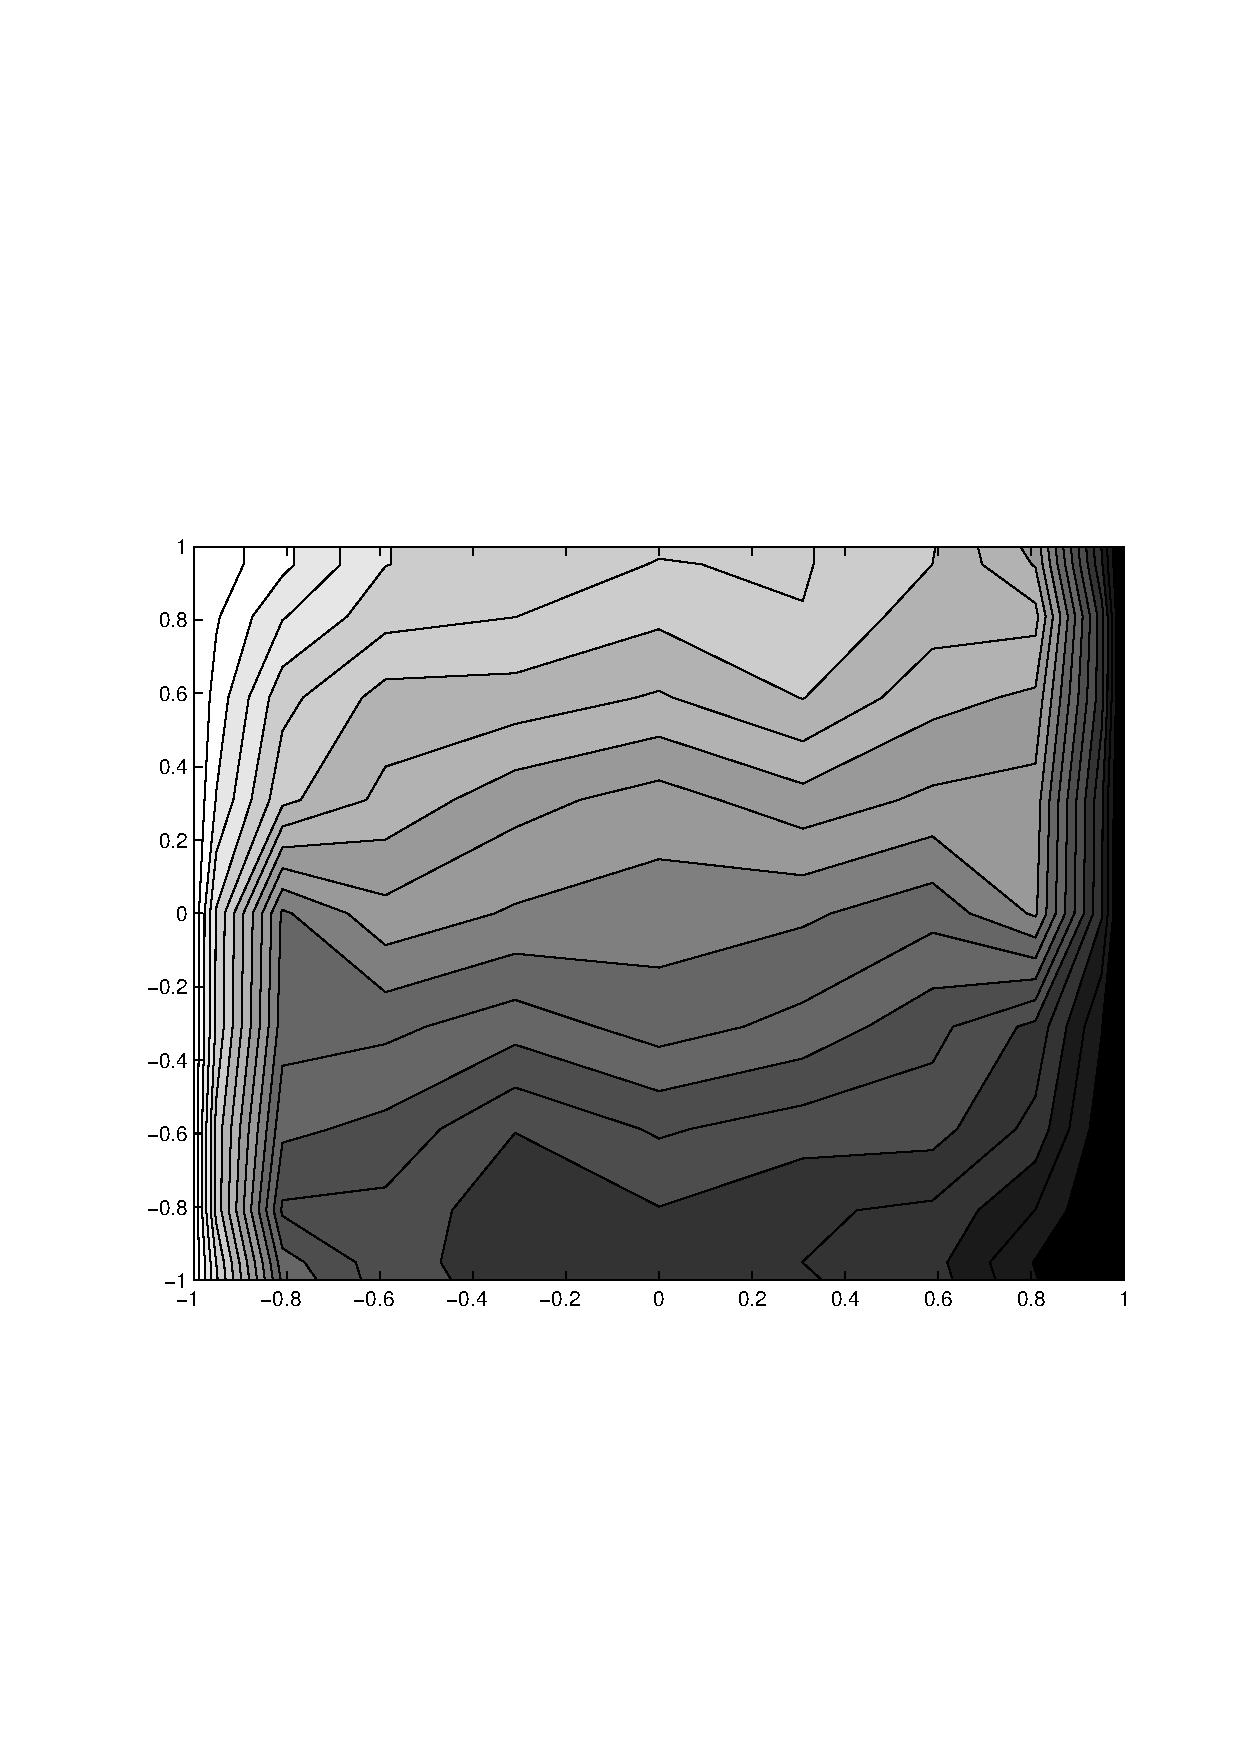
\includegraphics[scale=0.45, trim = 30mm 75mm 15mm 80mm,
clip]{./Figures/4-IVBP/temperature_t_5.pdf} \caption{Temperature contours, $t=0.5$.}
\end{figure}

\end{multicols}

\newpage

\begin{multicols}{2}

\begin{figure}[H]
\centering
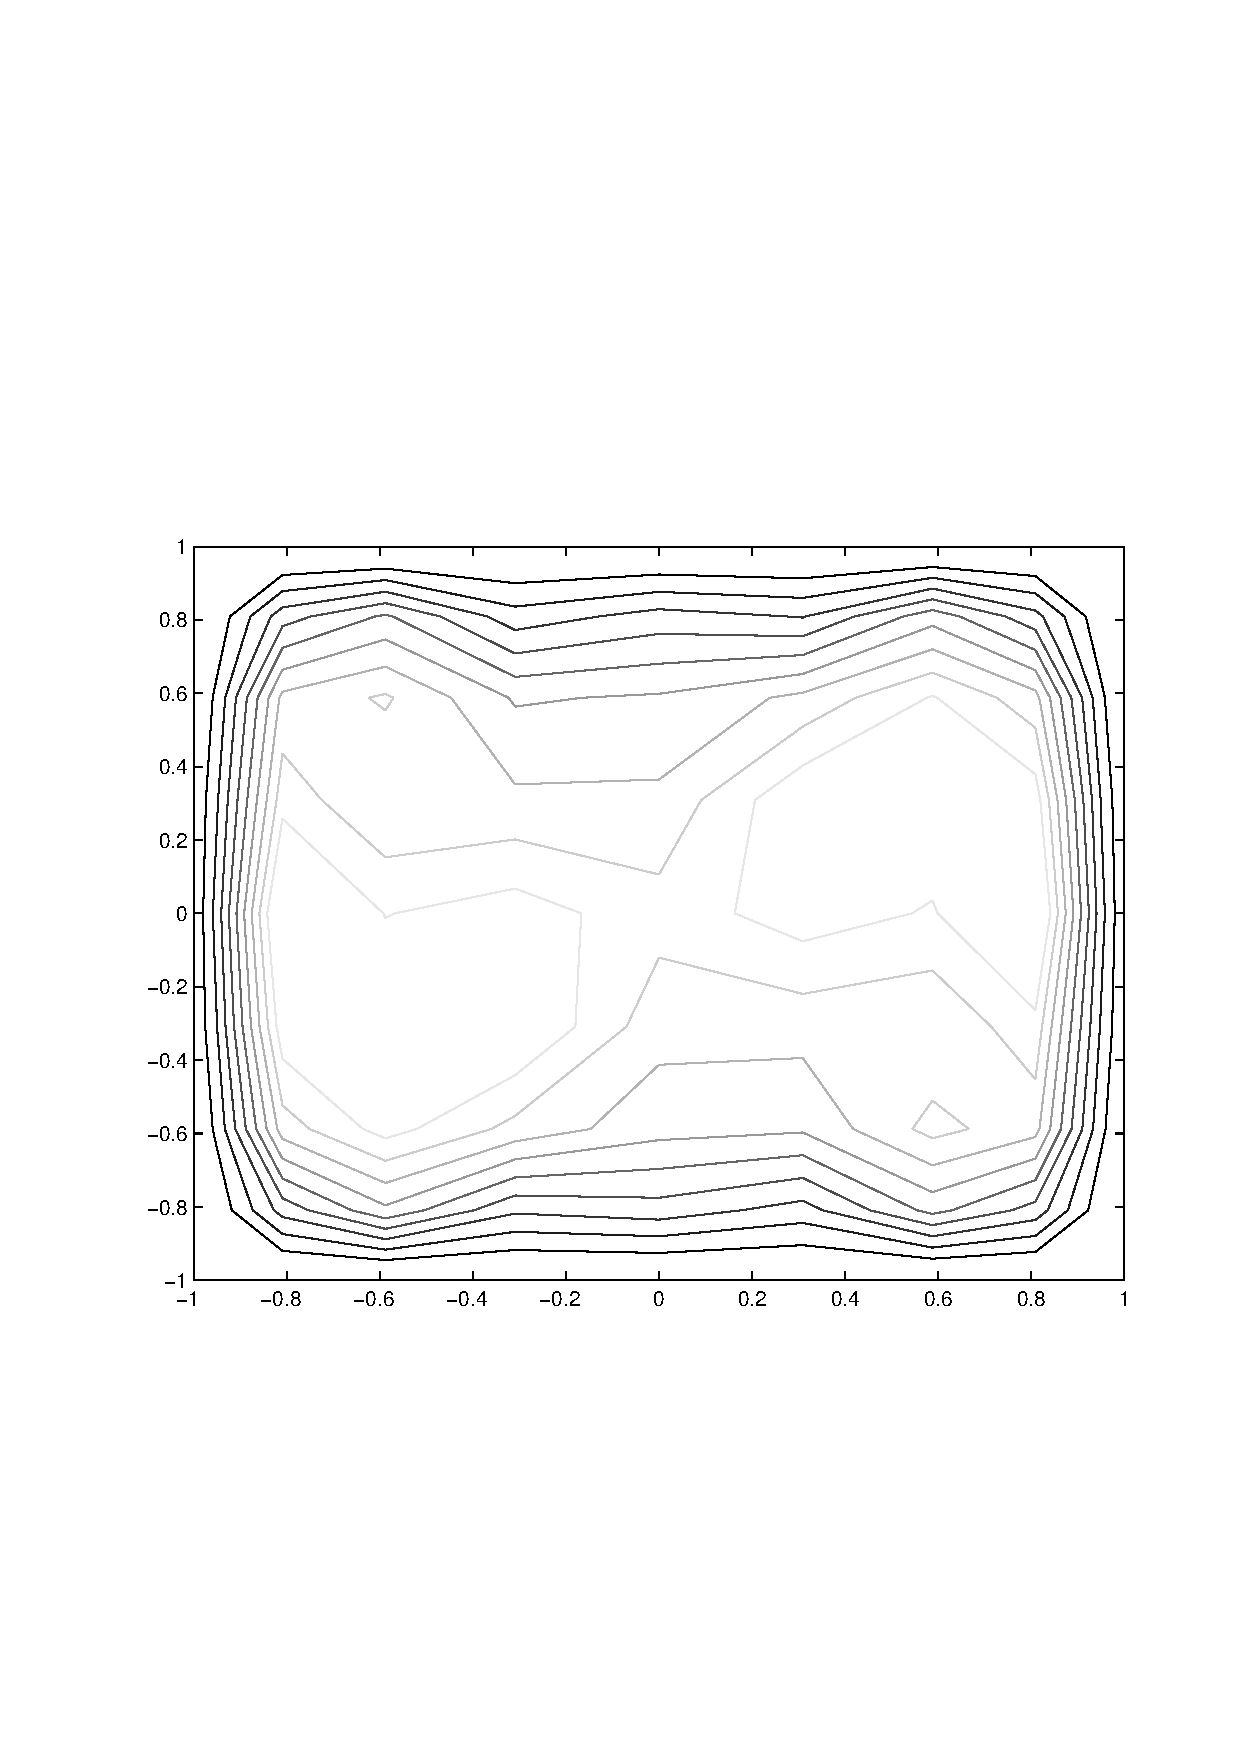
\includegraphics[scale=0.45, trim = 30mm 75mm 15mm 80mm, clip]{./Figures/4-IVBP/stream_t_8.pdf}
\caption{Stream function isolines, $t=0.8$.
}
\end{figure}


\columnbreak

\begin{figure}[H]
\centering
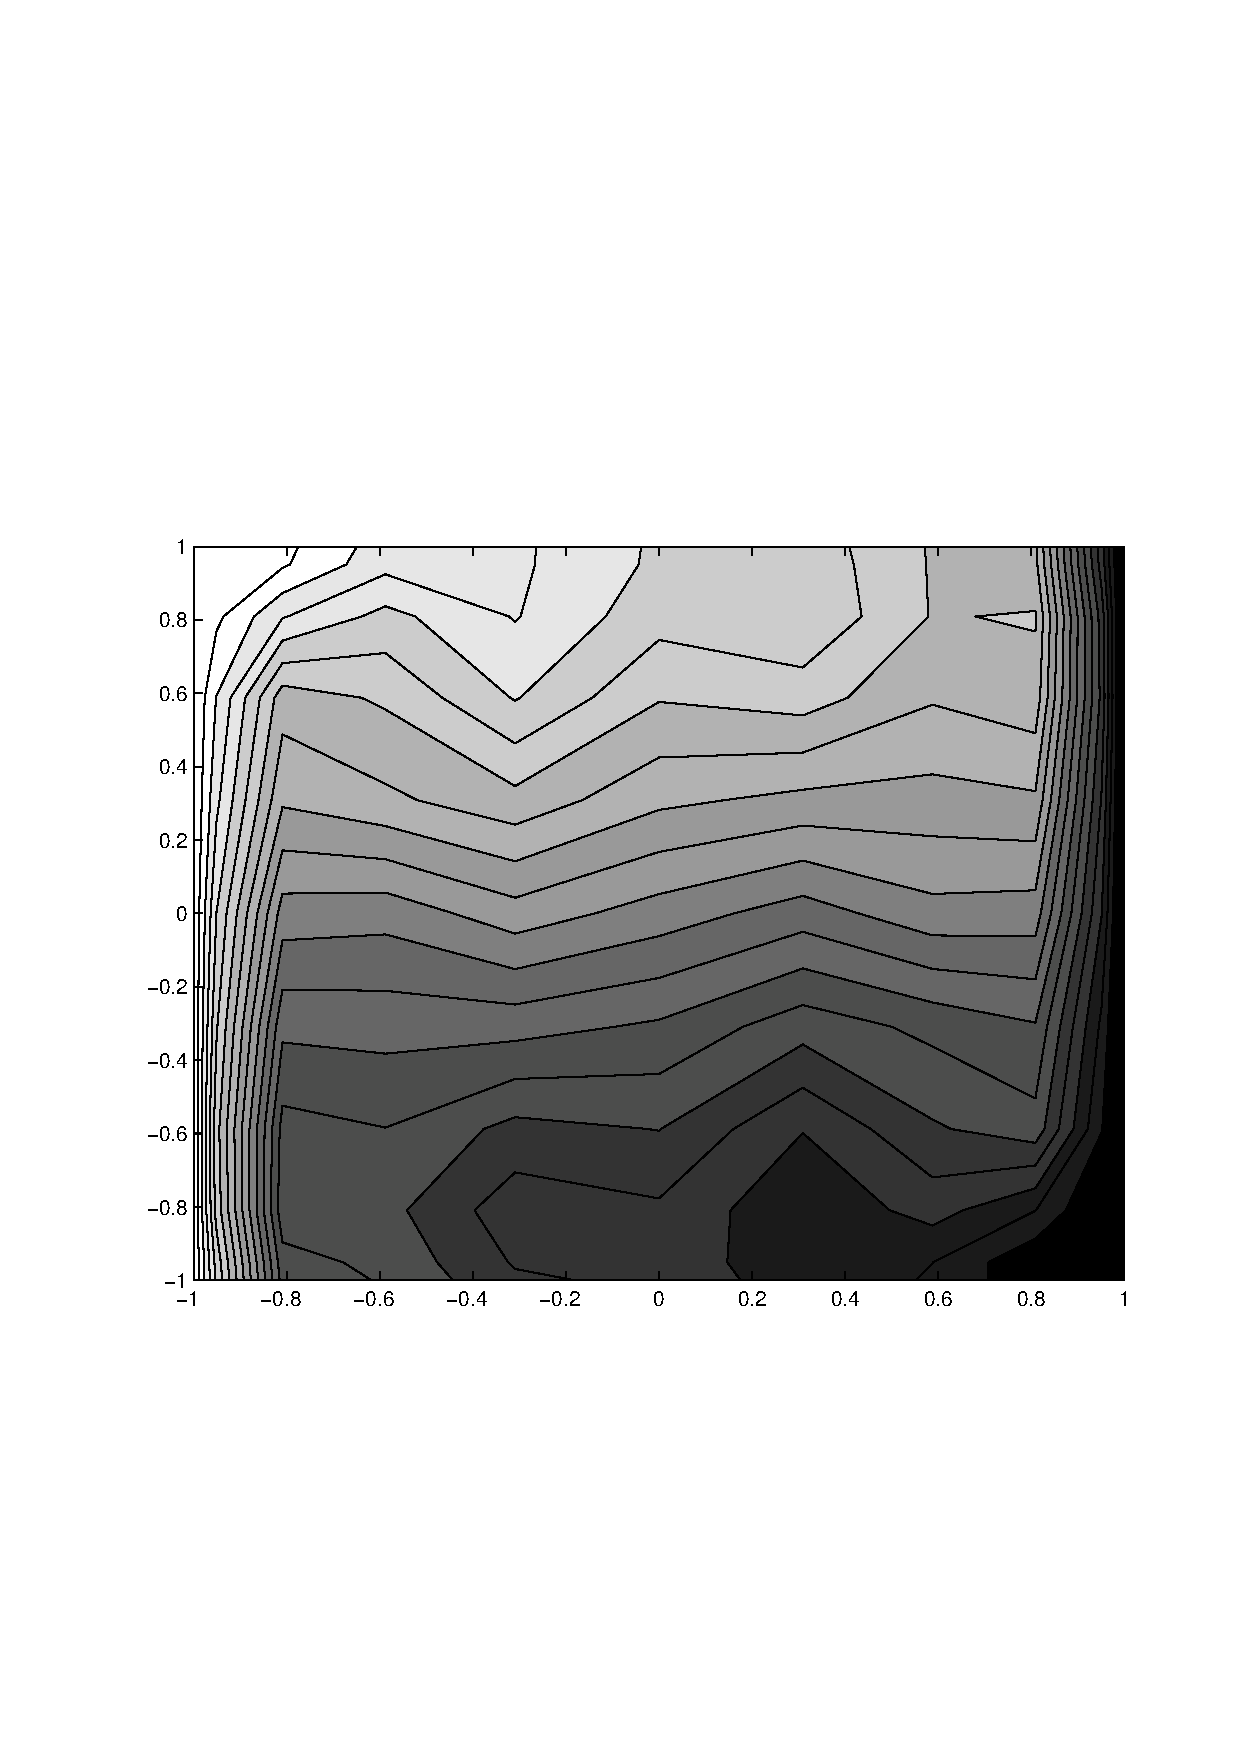
\includegraphics[scale=0.45, trim = 30mm 75mm 15mm 80mm,
clip]{./Figures/4-IVBP/temperature_t_8.pdf} \caption{Temperature contours, $t=0.8$.}
\end{figure}

\end{multicols}

\begin{multicols}{2}

\begin{figure}[H]
\centering
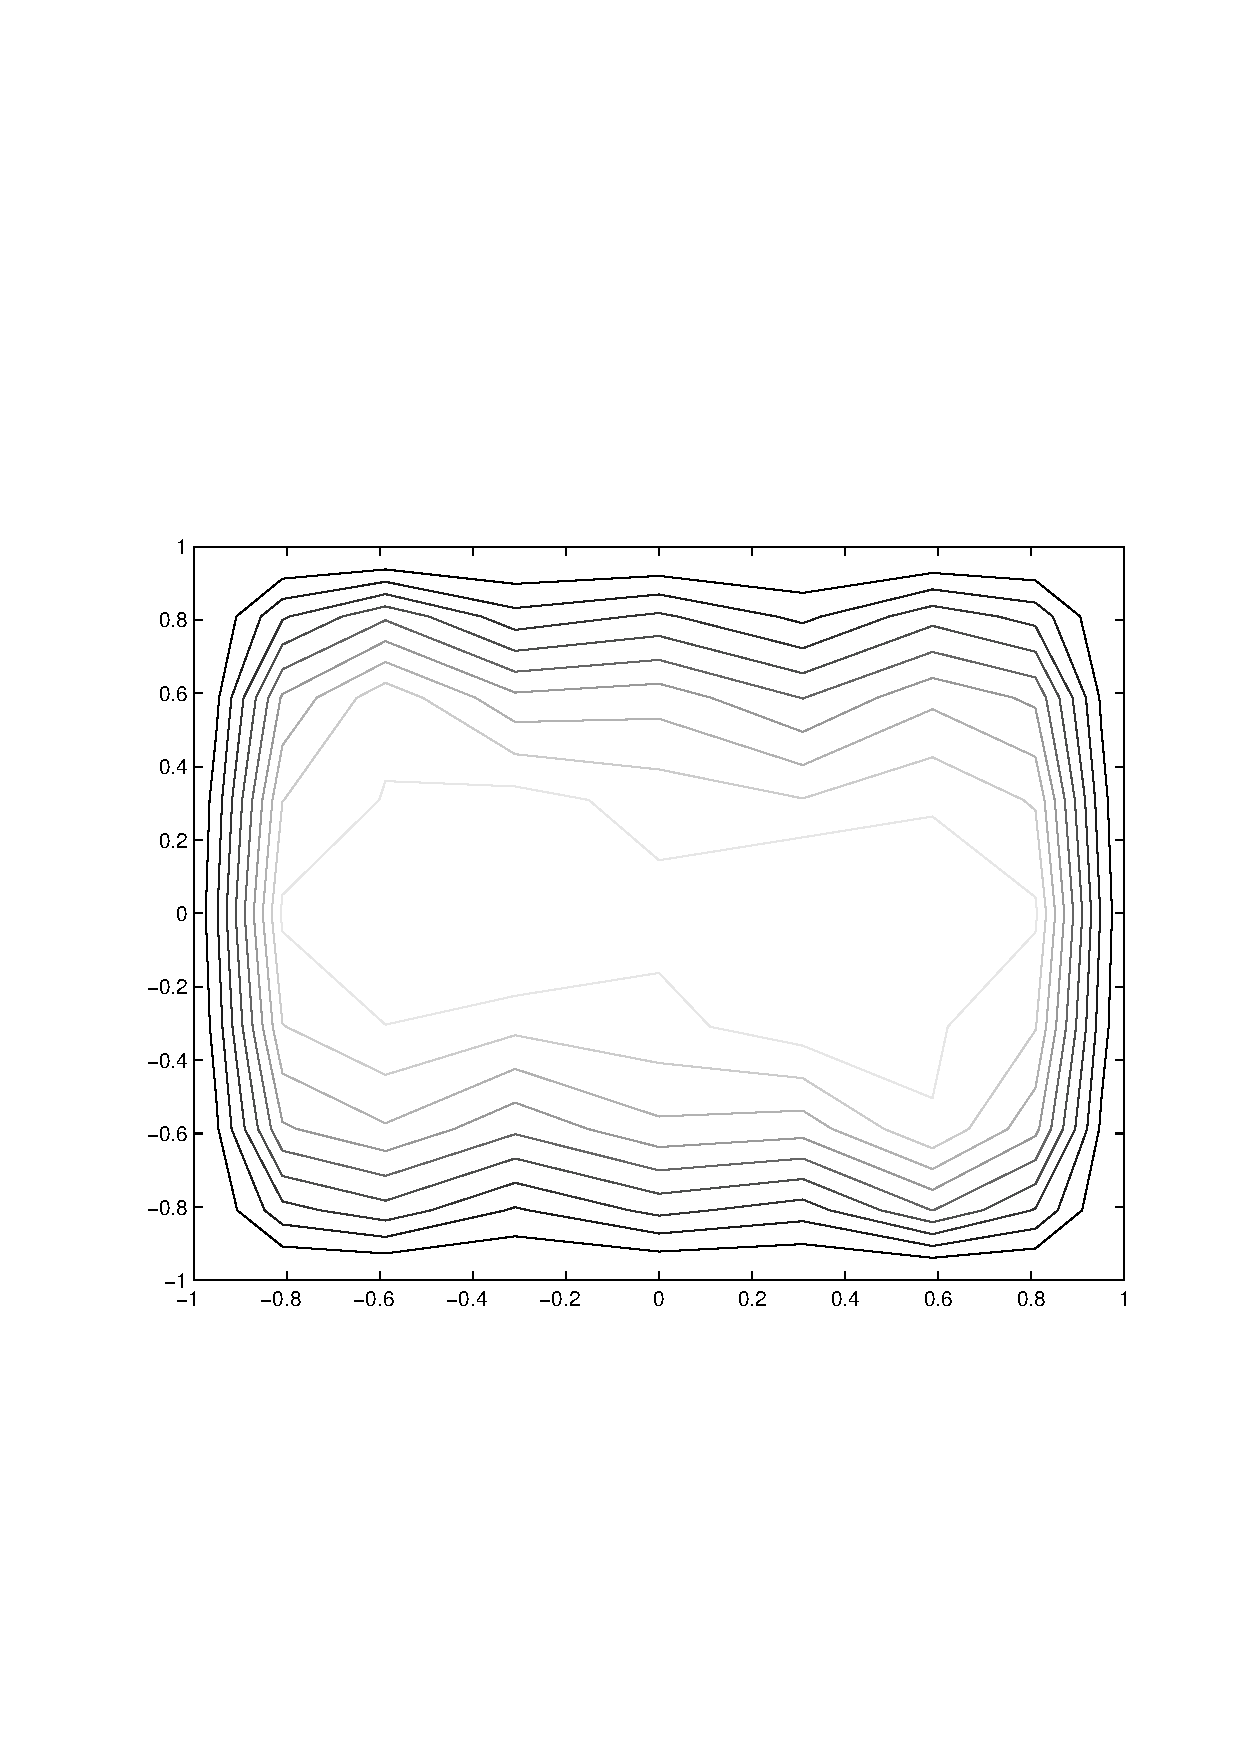
\includegraphics[scale=0.45, trim = 30mm 75mm 15mm 80mm, clip]{./Figures/4-IVBP/stream_t_10.pdf}
\caption{Stream function isolines, $t=1$.
}
\end{figure}


\columnbreak

\begin{figure}[H]
\centering
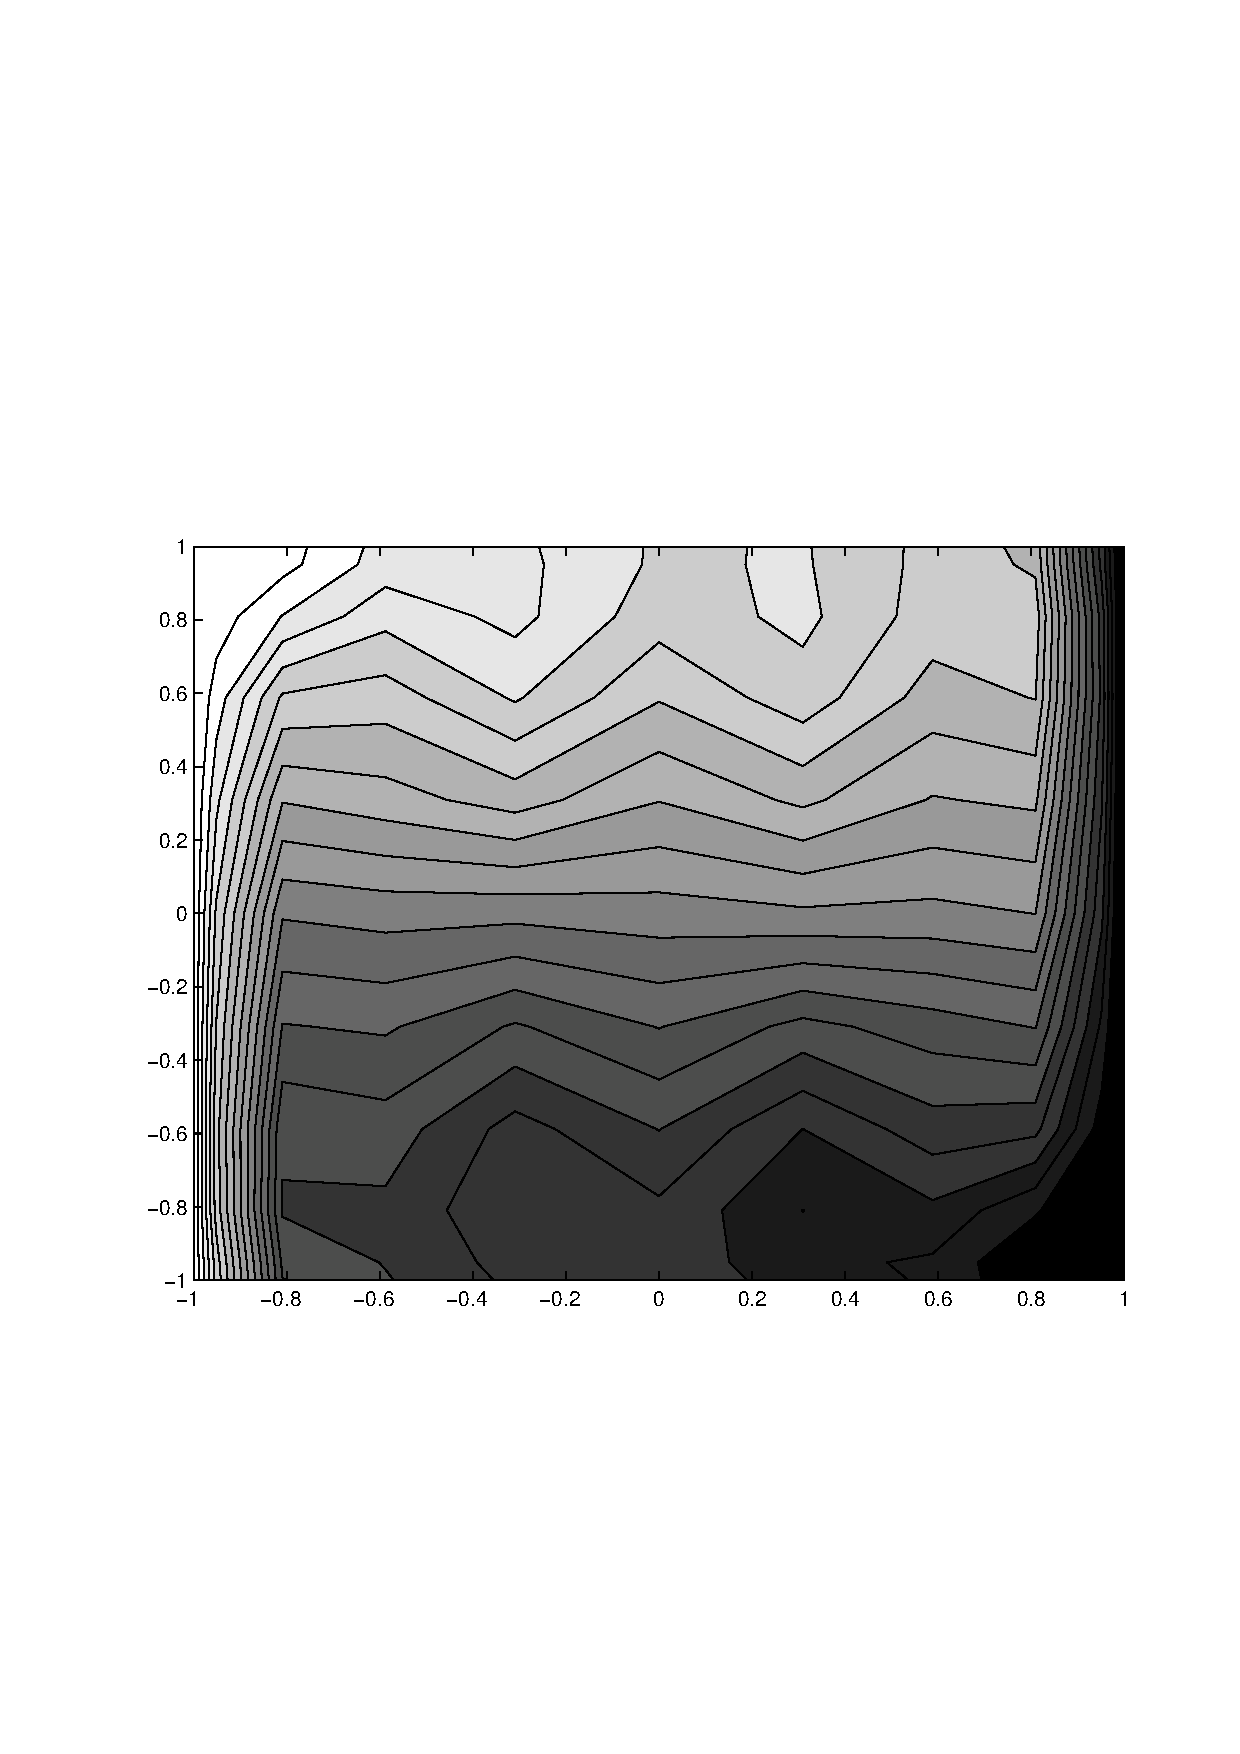
\includegraphics[scale=0.45, trim = 30mm 75mm 15mm 80mm,
clip]{./Figures/4-IVBP/temperature_t_10.pdf} \caption{Temperature contours, $t=1$.}
\end{figure}

\end{multicols}

\vspace{0.5cm}

\section{Convergence of the solution}

There are several techniques for evaluating the convergence of numerical
methods. Here we propose \textit{Richardson Extrapolation Method} for testing
our schemes. \\

\subsection{Richardson extrapolation}

This method is useful to test the convergence of the evolution problem. \\

One can assume that the exact solution (unknown) of the problem ($A$) can be
written as follows: 

\begin{equation}
A=A(h)+ K\cdot h^{\kappa} + K'\cdot h^{\kappa+1}+\ldots
\end{equation}

Where $A(h)$ is the numerical solution found when the time step is set to $h$;
and $\kappa$ is a parameter which depend on the temporal scheme used to solve
the problem ($\kappa=1$ with Euler's, Runge-Kutta:  $\kappa=4$). $K$ is
an unknown scalar.\\

One can also write: 

\begin{equation}
A=A(h)+ K\cdot h^{\kappa} + o(h^{\kappa+1})
\end{equation}

In order to evaluate the numerical convergence of the procedure, the program is
to be executed twice, with time steps set to $h$ and $h/2$. Two solutions are
obtained: $A(h)$ and $A(h/2)$: 

\begin{equation} \label{Richardson}
\begin{cases}
A=A(h)+ K\cdot h^{\kappa} + o(h^{\kappa+1})\\
A=A(h/2)+ K\cdot (h/2)^{\kappa} + o(h^{\kappa+1})
\end{cases}
\end{equation}

One can estimate the exact solution with these two equations: 

\begin{equation}
\begin{cases}
A=A(h)+ K\cdot h^{\kappa} + o(h^{\kappa+1})\\
2^{\kappa} \cdot A= 2^{\kappa}\cdot A(h/2)+ K\cdot (h)^{\kappa} +
o(h^{\kappa+1})
\end{cases}
\end{equation}

\begin{equation}
(2^{\kappa}-1) \cdot A= 2^{\kappa}\cdot A(h/2)- A(h) +
o(h^{\kappa+1})
\end{equation}

\begin{equation}
A= \frac{2^{\kappa}\cdot A(h/2)- A(h)}{(2^{\kappa}-1) } +
o(h^{\kappa+1})
\end{equation}

Then, the error for $h/2$ is: 

\begin{equation}
E(h/2) = A-A(h/2) = \frac{2^{\kappa}\cdot A(h/2)- A(h)}{(2^{\kappa}-1) } -
A(h/2)
\end{equation}

\begin{equation}
E(h/2) =  \frac{ A(h/2)- A(h)}{(2^{\kappa}-1) } 
\end{equation}

This easy procedure allows us to test the functioning of the numerical schemes
and the software application. Large errors indicate a strong dependence of the
solution with the time step, and the solution found is not trustable.\\

In the other hand, small errors give confidence to the method and the numerical
solution is more likely close to the exact solution.\\

As always, if we have an analytical solution, the goodness of the numerical
approach can be evaluated directly. \\

\newpage

If the error found does not satisfy our requirements a narrower time step
is required. It is easy to estimate the time step needed for a target error.
Going back to the equation \ref{Richardson}: 

\begin{equation}
A(h)-A(h/2)=-K\cdot (h^\kappa - (h/2)^\kappa)
\end{equation} 

\begin{equation}
K =-\frac{A(h)-A(h/2)}{ h^\kappa-(h/2)^\kappa }= \frac{A(h/2)-A(h)}{
h^\kappa \cdot(1-(1/2)^\kappa )}
\end{equation} \\

So the error can be calculated as follows,

\begin{equation}
E(h/2) = A-A(h/2) \simeq K(h/2)^\kappa+o(h^{\kappa+1})
\end{equation}

Then, 

\begin{equation}
E(h/2)  \simeq K(h/2)^\kappa
\end{equation}

With this equation we can set the time step to meet our requuirements. Let's
picture we want a precision lower than $1E-6$, then the time step needed is: 

\begin{equation}
h< 2 \cdot \left ( \frac{E(h/2)}{K}\right)^{1/\kappa}  
\end{equation}





